\documentclass[table]{beamer}
\usepackage{verbatim} % For using /begin{comment}; /end{comment}
\setbeamertemplate{footline}{%
    \raisebox{5pt}{\makebox[\paperwidth]{\hfill\makebox[10pt]{%
    \scriptsize\insertframenumber}}}}
\setbeamertemplate{navigation symbols}{}% Empty to get rid of them!
\setbeamertemplate{itemize items}[circle]
\setbeamertemplate{itemize subitems}[circle]
\usepackage{multirow}
\usepackage{textpos}
\usepackage{graphicx}
%\useoutertheme{infolines}
%\graphicspath{{images/}}
%\setbeamerfont{frametitle}{series=\bfseries} % Frame titles should be bold
\usepackage{lmodern}
\definecolor{oj}{rgb}{1.0,0.65,0.0}
\definecolor{cblue}{rgb}{0.39,0.58,0.93}
\definecolor{amethyst}{rgb}{0.6, 0.4, 0.8}
\definecolor{lightgrey}{rgb}{0.75, 0.75, 0.80}
\definecolor{tangerine}{rgb}{1.0, 0.6, 0.4}
\definecolor{arylyellow}{rgb}{0.91, 0.84, 0.42}
\definecolor{gsa}{rgb}{0.66, 0.89, 0.63}
\definecolor{aqua}{rgb}{0.5, 1.0, 0.83}
\definecolor{bblue}{rgb}{0.67, 0.9, 0.93}

%\usepackage{tikz}
%\usebackgroundtemplate{%
%\tikz\node[opacity=0.3]{%
%\setbeamercolor{background canvas}{bg=black}
%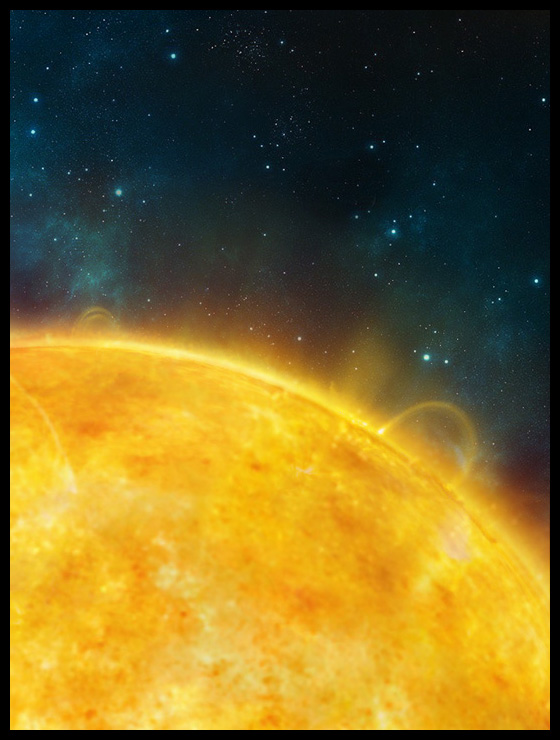
\includegraphics[height=\paperheight,width=\paperwidth]{awesome.jpg}};}

%\setbeamertemplate{background}{%
%\setbeamercolor{normal text}{bg=black, fg=white}
%\setbeamercolor{bgcolor}{fg=black,bg=red!20}
%\setbeamercolor{bgcolor}{bg=black}
%\setbeamercolor{bgcolor}{bg=red!20}

\setbeamercolor{background canvas}{bg=black}
\setbeamercolor{normal text}{fg=white}
\setbeamercolor{title}{fg=arylyellow}
\setbeamercolor{frametitle}{fg=tangerine}
\setbeamercolor{framesubtitle}{fg=gsa}
\setbeamercolor{block title}{fg=aqua}
\setbeamercolor{column title}{fg=aqua}
\setbeamercolor{description item}{fg=amethyst}
\setbeamercolor{itemize item}{fg=amethyst} % all frames will have red bullets
\setbeamercolor{itemize subitem}{fg=amethyst} % all frames will have red bullets
\setbeamercolor{enumerate item}{fg=amethyst} % all frames will have red bullets
\setbeamercolor{enumerate subitem}{fg=amethyst} % all frames will have red bullets

\newcommand\Wider[2][3em]{%
    \makebox[\linewidth][c]{%
       \begin{minipage}{\dimexpr\textwidth+#1\relax}
           \raggedright#2
       \end{minipage}%
    }%
}

\title{\textbf{Coronal Seismology}}
\subtitle{\textbf{ASTR 598}}
\date{\textbf{Spring 2016}}
\author{\textbf{Laurel Farris}}

\begin{document}
{\usebackgroundtemplate{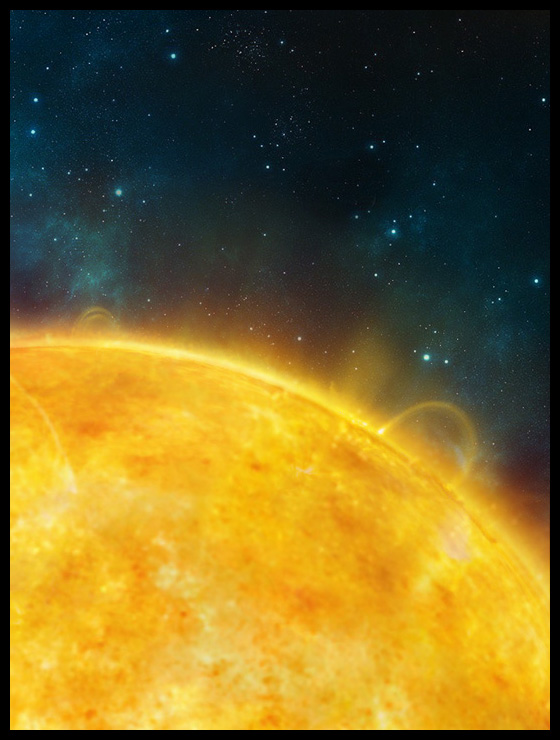
\includegraphics[width=\paperwidth]
    {awesome.jpg}}
\begin{frame}
    \titlepage{}
\end{frame}}%-------------------------------------------------------------%
\begin{frame}{Coronal seismology}{Technique and motivation}
    \begin{columns}
        %\column{0.5\paperwidth}
        \column{0.5\textwidth}
        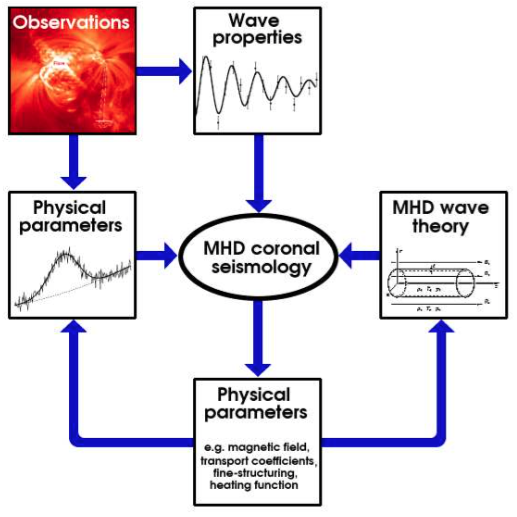
\includegraphics[width=\textwidth]{schematic.png}
        %\column{0.5\paperwidth}
        \column{0.5\textwidth}
            Elusive coronal properties:
            \begin{itemize}
                \item magnetic field strength, $\vec{B}$
                \item density, $\rho$
                \item Alfv\'en velocity, $V_A$
            \end{itemize}
            Solution: coronal seismology
            \begin{enumerate}
                \item Observe disturbances
                \item Measure properties
                \item Identify the wave or mode
                \item Extract coronal parameters
            \end{enumerate}
            Motivation:
            \begin{itemize}
                \item Coronal heating
                \item Space weather prediction
            \end{itemize}
    \end{columns}
\end{frame}%-------------------------------------------------------------%
\begin{frame}{Magnetohydrodynamics (MHD)}{Theory}
    %[Relationship between size and decay time].
    %[Something about Asc, TRACE, etc.]
    \begin{columns}
        \column{0.45\textwidth}
        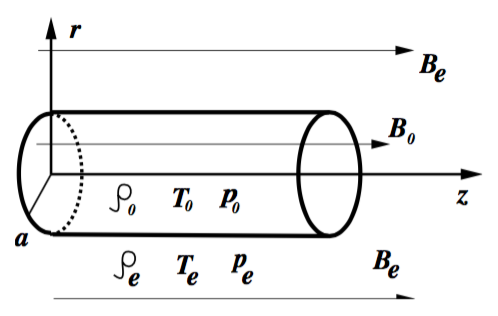
\includegraphics[width=\textwidth]{cylinder.png}\\
        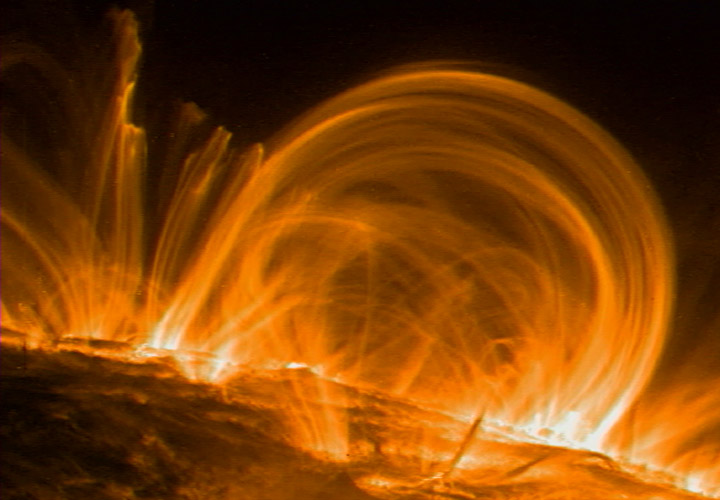
\includegraphics[width=\textwidth]{loop.jpg}
        \column{0.55\textwidth}
        Model:
        \begin{itemize}
            \item Straight flux tube in uniform magnetic field.
            \item Frozen-in plasma is compressive and elastic.
            %\item $ \xi(x) = \xi(r)e^{i(kz+m{\phi})} $
            \item Characteristic wave speeds are determined by
                $\rho$, $T$, $P$, and $\vec{B}$
        \end{itemize}
        \begin{enumerate}
            \item \textcolor{bblue}{Magnetoacoustic}
                $C_s = \sqrt{\frac{\gamma P}{\rho}}$
                \begin{enumerate}[(a)]
                    \item \textcolor{bblue}{Fast} $k_{A_0} < C_{fast} < C_{A_e} $
                    \item \textcolor{bblue}{Slow} $C_{T_0} < C_{slow} < C_{s_0} $
                \end{enumerate}
            \item \textcolor{bblue}{Alfv\'en}
                $V_A = \frac{B}{\sqrt{\mu_0\rho}}$
        \end{enumerate}
    \end{columns}
\end{frame}%-------------------------------------------------------------%
\begin{frame}{Dispersion diagram}{Phase speed ($v_{ph}=\frac{\omega}{k}$)
    as function of $ka$}
    \begin{figure}
        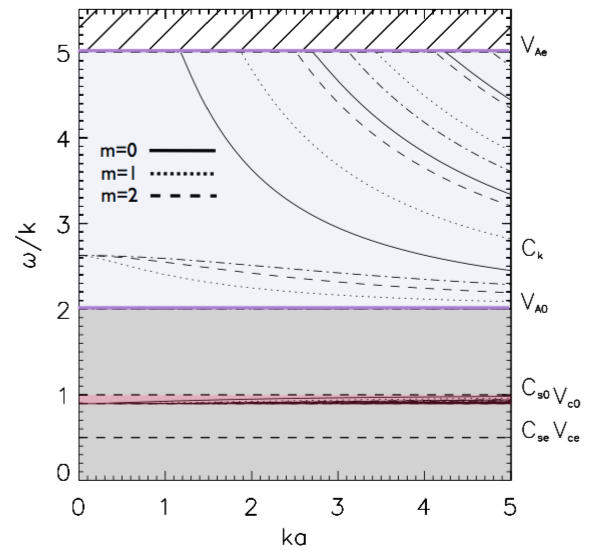
\includegraphics[width=0.65\paperwidth]{disp_diagram.png}
    \end{figure}
\end{frame}%-------------------------------------------------------------%
\begin{frame}{Research Topics}
    \begin{columns}
        \column{0.5\paperwidth}
        \column{0.5\paperwidth}
        \begin{enumerate}
            \item Kink oscillations
            \item Sausage oscillations
            \item Acoustic oscillations
            \item Propagating acoustic waves
            \item Propagating fast waves
            \item Torsional (Alfv\'en) modes
        \end{enumerate}
    \end{columns}
\end{frame}%-------------------------------------------------------------%
\begin{frame}[c]{Fast standing oscillations}{Kinks vs.\ Sausages}
    \begin{columns}
        \column{0.5\paperwidth}
        \begin{center}
            \framebox{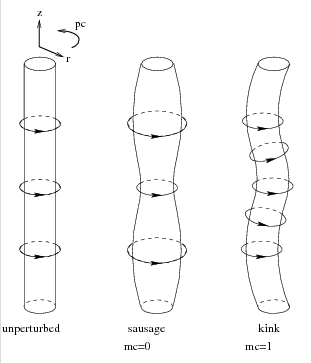
\includegraphics[width=0.8\textwidth]{kink_saus.png}}
        \end{center}
        \column{0.5\paperwidth}
        \vspace{-0.5in}
        \begin{block}{Kink}
            \begin{itemize}
                \item loop spatial displacement
                \item Asymmetric
                \item No intensity change
                \item $k\sigma \ll 1$, or $\sigma\ll\lambda$
                \item Derive magnetic field!
        \item Period $P=\frac{2L}{V_A}\sqrt{\frac{1+\rho_e/\rho_o}{2}}$
            where $\lambda=2L$ ($L$ is the loop length).
            Typically, $L \approx 60-600$ Mm in the corona.
            \end{itemize}
        \end{block}
        \begin{block}{Sausage}
            \begin{itemize}
                \item No loop spatial displacement
                \item Symmetric
                \item Intensity change\\ $\rightarrow$ density change
                \item $\lambda\sim\sigma$
                \item long-wavelength limit
            \end{itemize}
        \end{block}
\end{columns}
\end{frame}%-------------------------------------------------------------%
\begin{frame}{Standing oscillations vs.\ propagating waves}
    \begin{itemize}
        \item In loops, propagating waves damp before
            reaching opposite footpoint.
        \item Velocity and intensity are 90$^{\circ}$ out of phase
            for standing oscillations, and are in phase for propagating
            acoustic waves.
        \item Frequencies less than the cutoff are standing oscillations,
            waves with frequency greater than the cutoff propagate into
            the chromosphere.
    \end{itemize}
\end{frame}%-------------------------------------------------------------%
\begin{frame}{Torsional modes}{aka.\ Alfv\'en wave}
    Properties:
    \begin{itemize}
        \item m$=$0 (Axisymmetric, or azimuthally symmetric)
        \item transverse (shear) perturbations
        \item Parallel to $\vec{B}$
        \item Driving force: magnetic tensioin
        \item incompressible
        \item velocity: $v_{A} = \frac{B}{\mu_{o}\rho}$;
            $\sim$ 1000 km s$^{-1}$ in the corona
    \end{itemize}
    How to observe:
    \begin{itemize}
        \item Only get Doppler shifts from \emph{long}-period waves
            ($>$ a few minutes).
        \item Measure additional (i.e.\ non-thermal) broadening
            of coronal emission lines; indirect way to observe short-period waves.
        \item Spatial variation in Doppler shift for long periods.
            Gyrosynchrotron emission in radio regime.
    \end{itemize}
    Effects of twisting:
    \begin{itemize}
        \item Coupling of various MHD modes
    \end{itemize}
\end{frame}%-------------------------------------------------------------%
\begin{frame}{Examples from the literature}{A. K. Srivastava and B. N. Dwivedi}
    \begin{columns}
        \column{0.5\textwidth}
        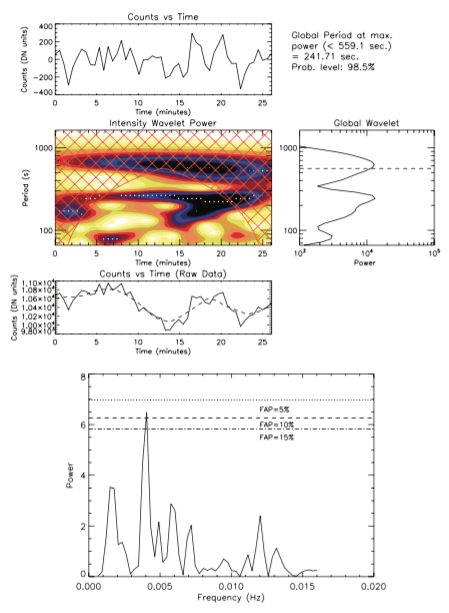
\includegraphics[width=\textwidth]{ex1.png}
        \column{0.5\textwidth}
        \begin{itemize}
            %\item Parallel to $\vec{B}$, perturbation of $\vec{B}$ is negligible.
            %\item Generated impulsively at one end of a footpoint.
            %\item Only penetrate $\sim$ 10\% into loop before
            %    damped by thermal conduction
            %\item weak dispersion in coronal conditions ($V_{A} \gg c_{s}$)
            %\item 3 phases: periodic, QP, decay
            %\item period = 3, 5, 10 minutes? Or 2--22 seconds? (see kink\_1),
            %\item velocity: 50--200 km s$^{-1}$
            %\item $c_{T} = \sqrt{\frac{c_{s}^2v_{A}^2}{c_{s}^2 + v_{A}^2}} $
            %    propagate sub-sonically at $c_{T}$, which is less than $c_{s}$
            %\item ``large'' amplitude, max in top of chromosphere
            %\item Observed using spectroscopy (intensity variations in
            %    EUV emission  and Doppler shifts)
            \item Observed bright point (BP) with EIS on \emph{HINODE}
            \item He{\footnotesize II} 256 \AA{} (TR and low corona)
            \item Fe{\footnotesize XV} 195 \AA{} (Upper corona)
            \item Leakage of acoustic oscillations in the inner corona
        \end{itemize}
    \end{columns}
\end{frame}%-------------------------------------------------------------%
\begin{frame}{Examples from the literature}{Authors}
    What observed and how, values measured, other parameters derived,
    mode identified, etc.
\end{frame}%-------------------------------------------------------------%
\begin{frame}{Examples from the literature}{Authors}
    What observed and how, values measured, other parameters derived,
    mode identified, etc.
\end{frame}%-------------------------------------------------------------%
\begin{frame}{Important Properties}
\begin{center}
    \begin{tabular}{c|c|c|c|}
    \cline{2-4} & {\textbf{period}} &
        {\textbf{decay time}} &
        {\textbf{velocity}}\\
    \hline \multicolumn{0}{|c|}{kink osc} &
        2--20 m & value & value\\
    \hline \multicolumn{0}{|c|}{sausage osc} &
        value & value & value\\
    \hline \multicolumn{0}{|c|}{acoustic osc} &
        20 m & 5--30 m & 200 km s$^{-1}$\\
    \hline \multicolumn{0}{|c|}{acoustic waves} &
        value & value & $<$150 km s$^{-1}$\\
    \hline \multicolumn{0}{|c|}{fast waves} &
        value & value & $>$150 km s$^{-1}$\\
    \hline \multicolumn{0}{|c|}{torsional modes} &
        10 m & value & 1000 km s$^{-1}$\\
    \hline
    \end{tabular}
\end{center}
\end{frame}%-------------------------------------------------------------%
{%
\setbeamercolor{background canvas}{bg=black}
\setbeamertemplate{background}{%
\parbox[c][\paperheight][c]{\paperwidth}{%
%\hspace{3cm}
\centering
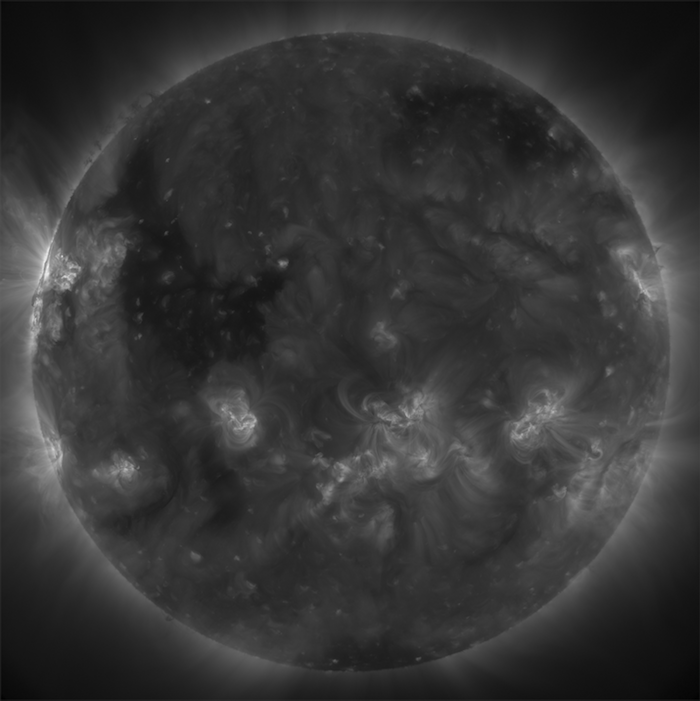
\includegraphics[height=\paperheight]{figures/full_disk.png}}}
\begin{frame}{Research}{AIA/SDO}
\end{frame}}%------------------------------------------------------------%
\begin{frame}
    Fe {\footnotesize XII, XXIV}\\
    193 \AA{}\\
    July 2012\\
    11--12 pm\\
\end{frame}

\begin{comment}
\begin{frame}[c]{Research}{[Looks nicer than white background]}
    \includegraphics[width=0.7\paperwidth]{figures/bp1.png}
\end{frame}%-------------------------------------------------------------%
\begin{frame}[c]{Research}
    \includegraphics[width=0.8\paperwidth]{figures/bp1_image.png}
\end{frame}%-------------------------------------------------------------%
\end{comment}%===========================================================%
\begin{frame}[c]{Research}
    \framebox{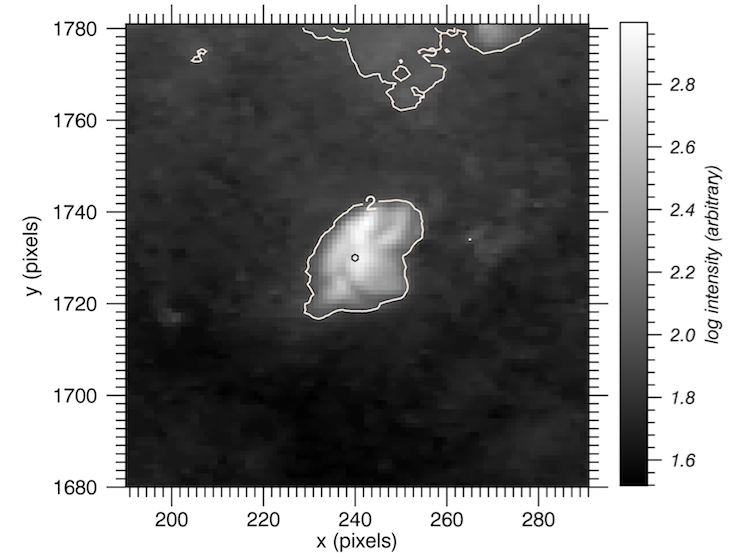
\includegraphics[width=0.8\paperwidth]{figures/bp1_contour.png}}
\end{frame}%-------------------------------------------------------------%
\begin{frame}{Research}
    \begin{center}
        \includegraphics[width=0.8\paperwidth]{figures/lightcurve3.png}
    \end{center}
\end{frame}%-------------------------------------------------------------%
\begin{frame}{Research}{Cross-correlations}
    \begin{block}{}
        \begin{columns}
            \column{0.3\textwidth}
            \includegraphics[width=0.2\paperwidth]{figures/bp1.png}
            \column{0.7\textwidth}
            [Cross-correlation example goes here.]
        \end{columns}
    \end{block}
    \begin{block}{}
    \Wider[4em]{%
    \begin{center}
        \framebox{\includegraphics[width=0.9\paperwidth]{figures/bp1_cool2.png}}
    \end{center}}
    \end{block}
\end{frame}%-------------------------------------------------------------%
\begin{frame}{Research}
    \begin{columns}
        \column{0.5\textwidth}
        \begin{block}{\centering Cross-correlation}
            \begin{center}
                \includegraphics[height=0.5\textheight]{figures/bp1_cc.png}
            \end{center}
        \end{block}
        \column{0.5\textwidth}
        \begin{block}{\centering Timelag}
            \begin{center}
                \includegraphics[height=0.5\textheight]{figures/bp1_tt2.png}
            \end{center}
        \end{block}
    \end{columns}
\end{frame}%-------------------------------------------------------------%
\begin{frame}{Future work}
    Other questions:
    \begin{itemize}
        \item What is the excitation mechanism for the observed
            disturbances?
        \item How are they damped, and what determines the timescales?
    \end{itemize}
    My future work:
    \begin{itemize}
        \item Download data in other wavelengths (i.e.\ coronal heights).
        \item Download data from other instruments,
            e.g.\ the Extreme Ultraviolet Variability Experiment
            (EVE) on SDO\@.
        \item Characterize other bright points in coronal hole,
            quiet sun, and active regions.
    \end{itemize}
\end{frame}%-------------------------------------------------------------%
\begin{frame}{Acknowledgements}
    Advisor: James McAteer
\end{frame}%-------------------------------------------------------------%

\begin{frame}{Extra slides here}
\end{frame}

\end{document}
